\subsection*{pulley4}

\begin{center}
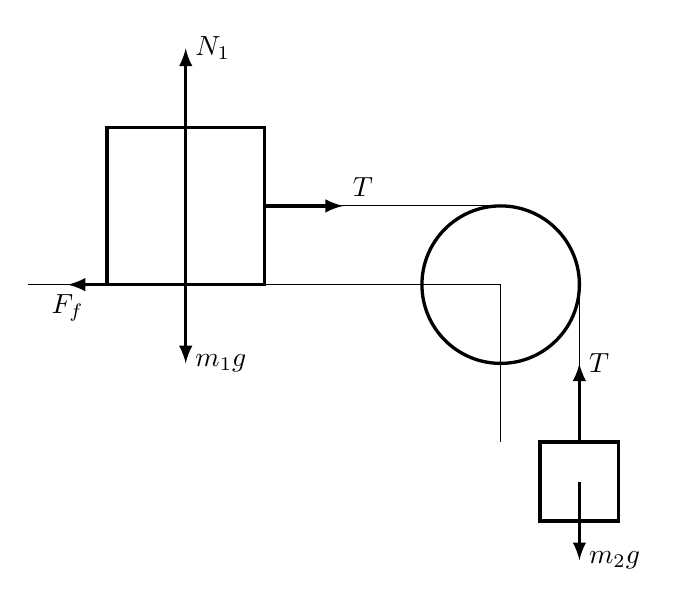
\begin{tikzpicture}

\draw (-6,0) -- (0,0) ;
\draw [very thick] (0,0) circle [radius=1] ;
\draw (1,0) -- (1,-2) ;
\draw (0,0) -- (0,-2) ;
\draw [very thick] (0.5,-3) rectangle (1.5,-2) ;
\draw (-3,1) -- (0,1) ;
\draw [very thick] (-5,0) rectangle (-3,2) ;
\draw [very thick, -{latex}] (-3,1) -- (-2,1) ;
\draw node at (-4,-1) [anchor=west] {$m_1g$} ;  
\draw [very thick, -{latex}] (1,-2.5) -- (1,-3.5) ;
\draw [very thick, -{latex}] (1,-2) -- (1,-1) ;
\draw node at (1,-3.5) [anchor=west] {$m_2g$} ;
\draw node at (1,-1) [anchor=west] {$T$} ;
\draw node at (-2,1) [anchor=south west] {$T$} ;
\draw [very thick, -{latex}] (-4,1) -- (-4,-1) ;
\draw [very thick, -{latex}] (-4,1) -- (-4,3) ;
\draw node at (-4,3) [anchor=west] {$N_1$} ;
\draw node at (-5.5,0) [anchor=north] {$F_f$} ;
\draw [very thick, -{latex}] (-4,0) -- (-5.5,0) ;
\end{tikzpicture}
\end{center}
